\chapter{Platform}
\label{chap:platform}

$Crowdy$ is an extensible general-purpose crowdsourcing platform to solve 
complex problems. The platform is developed over the fundamentals of stream 
processing paradigm in which a series of operations are applied to the continuous 
stream of data elements via operators.

$Crowdy$ is an operator-centric platform. Using this platform, a requester with no 
requirement of programming background can quickly translate a complex problem into 
a crowdsourcing application by simply selecting operators and connecting these operators 
together. Thanks to $Crowdy$'s focus on operators, requesters can design applications 
by selecting right set of building blocks that are necessary to solve a complex problem 
and customizing these blocks particular to the computation to-be-conducted.

$Crowdy$ embodies several features:
\begin{itemize}
	\item A standard toolkit of operators that can employ computation resources 
	(human or software) to accomplish various tasks
	\item Configuration support to design coordination of computation resources 
	over operators
	\item Operator parameterization and customization for support of customizable 
	collaborations
	\item Application runtime interface
\end{itemize}

In the remainder of this chapter, the fundamental concepts of $Crowdy$ are explained 
in more detail and features are explored as we look into various aspects of application 
development using $Crowdy$ platform.

\section{A "Hello World" application}
$Crowdy$ applications are developed to solve complex and sophisticated problems 
that require both human intelligence and computing power. A typical application contains 
three main high-level components: data ingest, processing and data egress.

Let's consider a minimal "Hello World" application that has these three components 
in total, connected in a simple pipeline topology. Figure~\ref{fig:helloworld} demonstrates 
the application in the form of a flow graph. On the ingest side, there is a 
\textit{source operator}, which, acts like a data generator. Source operator produces 
data tuples that are processed down the flow by the 
\textit{processing operator}. Finally, the \textit{sink operator} simply converts the tuples i
n such a form (text file, email etc) that can be easily interpreted by requesters.

The application flow graph is specified as a series of operator instances and connections 
(data flows) that link them. A data flow basically transfers data tuples 
produced by an operator to another. One or more data segments can be assembled in a 
data tuple via output specification of operator instance. In addition, several options can 
be specified to configure operator instance. These include parameters, operator-specific 
rules, which is studied in the rest of this chapter.

\begin{figure}[ht]
	\centering
	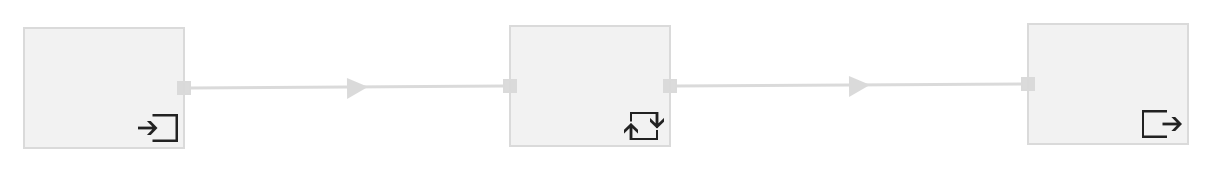
\includegraphics[width=0.85\textwidth]{figures/helloworld.png}
	\caption{A sample, minimal $Crowdy$ application.}
	\label{fig:helloworld}
\end{figure}

In a more realistic application, one or more source operators can be employed to produce 
various data tuples that differ in both size and specification. Similarly, the application would 
have one or more processing operators along with other types of operators organized in a way 
that is significantly more complex than this example.

\section{Operator}
An operator is the basic building block of an application. As soon as an operator is created, 
a unique ID is generated and assigned to it. Operator has a type that is specified at the time of 
creation, and type determines configuration respectively. In addition, operator has optional 
name and description fields that can be used for bookkeeping purposes.

Operator may have an input port or output port or both corresponding to it's type 
definition. Figure~\ref{fig:basicoperator} demonstrates a base operator, which 
consists of a body and ports. Although it is not shown here, each operator presentation 
has a specific icon on their body associated to it's type.

\begin{figure}[ht]
	\centering
	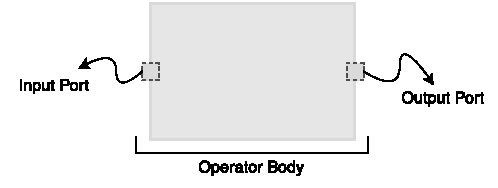
\includegraphics[width=0.5\textwidth]{figures/basicoperator.pdf}
	\caption{Base operator representation.}
	\label{fig:basicoperator}
\end{figure}

$Crowdy$ provides a set of built-in operators that can be used to build applications. 
In general, these operators perform common tasks associated with data generation, 
processing and outputting and are generally cross-domain. These operators can be 
grouped into six main categories: \textit{source, sink, processing, relational, utility, adapter}.

\subsection{Source operators}
The set of source operators generates data tuples. These operators do not have 
an input port, but have an output port, which outputs data tuples. Figure~\ref{fig:sourceoperator} 
represents a source operator.

\begin{figure}[ht]
	\centering
	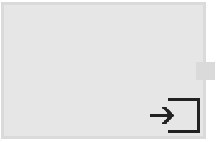
\includegraphics[width=0.25\textwidth]{figures/SourceOperator.pdf}
	\caption{Source operator representation.}
	\label{fig:sourceoperator}
\end{figure}

Source operators together with processing operators are the ones that can be 
used to specify data flow coming out of an operator. Output specification is an 
action to identify the data tuple with a series of segments. Other operator types 
cannot make changes on output specification, but manipulate the flow by dropping 
or copying data tuples.

\textbf{human.} 
The \textit{human source operator} is a stateless operator used to produce new data tuples 
via human workers. Existing crowdsourcing services such as MTurk is used 
to produce new tuples over the results retrieved from human intelligent tasks. These 
tasks are automatically created and posted with respect to the specified parameters 
of the operator.

Human source operator has the following parameters:
\begin{itemize}
	\item \texttt{number of copies}: The maximum number of data tuples can be 
	generated by the operator. It's value ranges from 1 to 1000.
	\item \texttt{max allotted time}: The maximum time in seconds given to a human 
	worker to solve and submit the task. It's value ranges from 10 to 300.
	\item \texttt{payment}: The payment in cents to be given to the human worker in 
	case of successful task completion. It's value ranges from 5 to 500.
	\item \texttt{instructions}: The detailed information for human workers on how to 
	complete the task.
	\item \texttt{question}: The actual sentence asking for specific information.
	\item \texttt{input list}: The list of \texttt{input}s that will be shown to human worker to fill.
\end{itemize}

An \texttt{input} can be a type of \textit{text, number, single choice} or 
\textit{multiple choice}. A text-input presents an input field where the human worker can 
enter data. The maximum number of characters that can be entered to the field can be 
set by the requester. Similarly number-input corresponds to a input field where only 
numbers can be fed in, and the maximum and minimum value for the field are set by 
the requester. The other two input types conform to input fields where the options given 
by the requester are presented to the human worker as a list. Human worker is expected 
to select only one and one or more options for single choice and multiple choice types 
respectively.

%This operator has a significant role in the platform. 
% platform-independence, abstracts away the details of the underlying platform
% use results of other operators
% customize collaboration by specifying audience

\textbf{manual.}
The \textit{manual source operator} is another stateless operator to produce new data 
tuples. However, this operator uses manually entered text to create new tuples. Operator 
retrieves the manual text, parses it line by line and then applies delimiter if selected. 
Therefore, each line constitutes a data tuple, and delimiter is used to create segments 
within a tuple.

Manual source operator has the following parameters:
\begin{itemize}
	\item \texttt{manual entry}: The manual text to be parsed and used to produce 
	new tuples.
	\item \texttt{delimiter}: Delimiter to determine segments in a tuple. This can be one 
	of the following values: none, white space, tab, comma, column.
\end{itemize}

\subsection{Sink operators}
The set of sink operators generates data tuples. These operators do not have 
an input port, but have an output port, which outputs data tuples. Figure~\ref{fig:sinkoperator} 
represents a source operator.

\begin{figure}[ht]
	\centering
	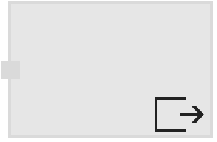
\includegraphics[width=0.25\textwidth]{figures/SinkOperator.pdf}
	\caption{Sink operator representation.}
	\label{fig:sinkoperator}
\end{figure}

\subsection{Processing operators}
TODO

\subsection{Relational operators}
TODO

\subsection{Utility operators}
TODO

\section{Flow compositon}
TODO